\documentclass[msc, noindex, hyperref, entetes, prelimtm, francais]{theseINRS} % Pour une thèse de doctorat, remplacer "msc" par "phd"

\usepackage[utf8]{inputenc} % Pour pouvoir taper les accent directement et sans passer par \'
\usepackage[T1]{fontenc} % Pour que les accents soient correctement traités dans le PDF
\usepackage{lmodern} % Pour que les accents soient correctement traités dans le PDF
\usepackage{amsmath} % Pour offrir plus de symboles mathématiques
\usepackage{natbib} % Pour citer des références avec \cite et \citep
\usepackage[letterpaper, margin=25mm]{geometry} % Pour la définition de la mise en forme du document
\usepackage{graphicx} % Pour insérer des images avec la commande \includegraphics
\usepackage[figuresright]{rotating} % Pour inclure des éléments en mode paysage en conservant les entêtes en mode portrait (environnement sideways)
\usepackage{tabularx} % Pour rendre plus flexible la création de tableaux
\usepackage{nomencl} % Pour générer une liste d'abréviations
\usepackage[font={singlespacing,footnotesize,bf}]{caption} % Pour définir le style des légendes de figures
\usepackage[font={singlespacing,footnotesize}]{subcaption} % Pour générer des sous-figures (subfig is deprecated)
\usepackage{textcomp} % Pour que les symboles de degrés apparaissent plus beaux
\usepackage{emptypage} % Pour enlever les numéros de page sur les pages blanches

\raggedbottom % Pour uniformiser l'espacement vertical entre les éléments dans les pages

%%%%%%%%%%%%%%%%%%%%%%%%%%%%%%%%%%%%%%%%%%%%%%%%%%%%%%%%%%

\begin{document}
\shorthandoff{:} % Ne pas ajouter automatiquement un espace avant un ":"
\shorthandoff{;} % Ne pas ajouter automatiquement un espace avant un ";"
\shorthandoff{?} % Ne pas ajouter automatiquement un espace avant un "?"
\shorthandoff{!} % Ne pas ajouter automatiquement un espace avant un "!"

\pagesprelim
\PrenomNom{Prénom Nom}
\titre{TITRE EN LETTRES MAJUSCULES} % en lettres majuscules
%\soustitre{Sous-titre} % Si désiré, ajouter un sous-titre
\programme{sciences de l'eau}
\grade{\textit{Maître es Sciences}, M.Sc.}
\jury{Examinateur externe &  Prénom Nom\\
	& Affiliation \\[0.5cm]
	Examinateur interne & Prénom Nom \\
	& Affiliation \\[0.5cm]
	Directeur de recherche & Prénom Nom \\
	& Affiliation \\[0.5cm]}
\annee{Année}

\maketitle

%\include{dedicace/dedicace} % Section facultative
%!TEX root = ../main.tex
\chapter*{Remerciements}
\addcontentsline{toc}{chapter}{Remerciements} % Ajouter à la table des matières.

Lorem ipsum dolor sit amet, consectetur adipiscing elit. Sed tortor quam, facilisis in magna at, convallis fringilla risus. Curabitur adipiscing imperdiet ligula ut congue. Nunc non urna sed velit aliquet tempor. Fusce tempus vestibulum pharetra. Sed laoreet erat sed odio cursus, et egestas lacus fringilla. Nullam sollicitudin condimentum scelerisque. Morbi fermentum blandit purus, eget feugiat quam egestas at. Nam at velit ac velit feugiat lacinia. Mauris quis tortor dignissim, feugiat justo eget, interdum tortor. Proin vel lacus non eros eleifend aliquet nec at elit. Integer rhoncus laoreet ligula.

Phasellus vitae orci ac tellus accumsan rutrum et rutrum elit. Phasellus accumsan nunc quam, a bibendum felis posuere quis. Ut dui turpis, consequat sit amet felis in, imperdiet aliquam elit. Aliquam eget iaculis nisl, eu lobortis eros. Nunc euismod eros eu felis tristique congue. Morbi aliquam sapien lacus, non viverra eros venenatis sit amet. Aliquam erat volutpat. Vestibulum arcu elit, fringilla in ornare in, mattis sed nisl. Nunc cursus sem odio, at convallis nulla egestas vitae. Sed euismod semper ante eget egestas. Nulla aliquam nisl eu dui lobortis, sed euismod sem tincidunt. Proin laoreet risus dolor, vel commodo turpis lobortis eu. Quisque luctus at arcu eget hendrerit. Sed dapibus risus condimentum mauris accumsan, a scelerisque lorem tristique. Duis at vulputate augue. Integer diam mauris, condimentum eu odio sed, pellentesque gravida odio.

Donec vitae malesuada odio. Vestibulum ante ipsum primis in faucibus orci luctus et ultrices posuere cubilia Curae; Fusce est massa, aliquet ut cursus quis, porttitor at leo. Etiam consectetur nulla mi, et ultricies tortor elementum eget. Vestibulum in purus accumsan, ullamcorper libero in, rutrum risus. Quisque non pellentesque mi. In hac habitasse platea dictumst. Sed facilisis non dolor quis porta. Vivamus ornare eget sem nec sollicitudin. Ut a purus fringilla, fringilla elit et, varius lectus. Proin et mauris odio.

Sed tincidunt semper pharetra. Sed sodales erat in tristique interdum. Interdum et malesuada fames ac ante ipsum primis in faucibus. Integer bibendum lorem ipsum, vel dapibus dolor semper convallis. Sed vitae orci vitae lacus elementum pellentesque. Pellentesque tincidunt odio et purus placerat, id vulputate nulla convallis. Fusce pellentesque egestas enim, vitae tempor nulla egestas eget. Donec pretium ipsum vitae egestas dapibus.
 % Section facultative (Remerciements ou Avant propos, pas les deux)
%\include{avPropos/avPropos} % Section facultative (Remerciements ou Avant propos, pas les deux)
%!TEX root = ../main.tex
\chapter*{Résumé}
\addcontentsline{toc}{chapter}{Résumé} % Ajouter à la table des matières.

Lorem ipsum dolor sit amet, consectetur adipiscing elit. Sed tortor quam, facilisis in magna at, convallis fringilla risus. Curabitur adipiscing imperdiet ligula ut congue. Nunc non urna sed velit aliquet tempor. Fusce tempus vestibulum pharetra. Sed laoreet erat sed odio cursus, et egestas lacus fringilla. Nullam sollicitudin condimentum scelerisque. Morbi fermentum blandit purus, eget feugiat quam egestas at. Nam at velit ac velit feugiat lacinia. Mauris quis tortor dignissim, feugiat justo eget, interdum tortor. Proin vel lacus non eros eleifend aliquet nec at elit. Integer rhoncus laoreet ligula.

Phasellus vitae orci ac tellus accumsan rutrum et rutrum elit. Phasellus accumsan nunc quam, a bibendum felis posuere quis. Ut dui turpis, consequat sit amet felis in, imperdiet aliquam elit. Aliquam eget iaculis nisl, eu lobortis eros. Nunc euismod eros eu felis tristique congue. Morbi aliquam sapien lacus, non viverra eros venenatis sit amet. Aliquam erat volutpat. Vestibulum arcu elit, fringilla in ornare in, mattis sed nisl. Nunc cursus sem odio, at convallis nulla egestas vitae. Sed euismod semper ante eget egestas. Nulla aliquam nisl eu dui lobortis, sed euismod sem tincidunt. Proin laoreet risus dolor, vel commodo turpis lobortis eu. Quisque luctus at arcu eget hendrerit. Sed dapibus risus condimentum mauris accumsan, a scelerisque lorem tristique. Duis at vulputate augue. Integer diam mauris, condimentum eu odio sed, pellentesque gravida odio.

Donec vitae malesuada odio. Vestibulum ante ipsum primis in faucibus orci luctus et ultrices posuere cubilia Curae; Fusce est massa, aliquet ut cursus quis, porttitor at leo. Etiam consectetur nulla mi, et ultricies tortor elementum eget. Vestibulum in purus accumsan, ullamcorper libero in, rutrum risus. Quisque non pellentesque mi. In hac habitasse platea dictumst. Sed facilisis non dolor quis porta. Vivamus ornare eget sem nec sollicitudin. Ut a purus fringilla, fringilla elit et, varius lectus. Proin et mauris odio.

Sed tincidunt semper pharetra. Sed sodales erat in tristique interdum. Interdum et malesuada fames ac ante ipsum primis in faucibus. Integer bibendum lorem ipsum, vel dapibus dolor semper convallis. Sed vitae orci vitae lacus elementum pellentesque. Pellentesque tincidunt odio et purus placerat, id vulputate nulla convallis. Fusce pellentesque egestas enim, vitae tempor nulla egestas eget. Donec pretium ipsum vitae egestas dapibus.

\textbf{Mots-clés} Lorem ipsum

\chapter*{Abstract}
\addcontentsline{toc}{chapter}{Abstract} % Ajouter à la table des matières.

Lorem ipsum dolor sit amet, consectetur adipiscing elit. Sed tortor quam, facilisis in magna at, convallis fringilla risus. Curabitur adipiscing imperdiet ligula ut congue. Nunc non urna sed velit aliquet tempor. Fusce tempus vestibulum pharetra. Sed laoreet erat sed odio cursus, et egestas lacus fringilla. Nullam sollicitudin condimentum scelerisque. Morbi fermentum blandit purus, eget feugiat quam egestas at. Nam at velit ac velit feugiat lacinia. Mauris quis tortor dignissim, feugiat justo eget, interdum tortor. Proin vel lacus non eros eleifend aliquet nec at elit. Integer rhoncus laoreet ligula.

Phasellus vitae orci ac tellus accumsan rutrum et rutrum elit. Phasellus accumsan nunc quam, a bibendum felis posuere quis. Ut dui turpis, consequat sit amet felis in, imperdiet aliquam elit. Aliquam eget iaculis nisl, eu lobortis eros. Nunc euismod eros eu felis tristique congue. Morbi aliquam sapien lacus, non viverra eros venenatis sit amet. Aliquam erat volutpat. Vestibulum arcu elit, fringilla in ornare in, mattis sed nisl. Nunc cursus sem odio, at convallis nulla egestas vitae. Sed euismod semper ante eget egestas. Nulla aliquam nisl eu dui lobortis, sed euismod sem tincidunt. Proin laoreet risus dolor, vel commodo turpis lobortis eu. Quisque luctus at arcu eget hendrerit. Sed dapibus risus condimentum mauris accumsan, a scelerisque lorem tristique. Duis at vulputate augue. Integer diam mauris, condimentum eu odio sed, pellentesque gravida odio.

Donec vitae malesuada odio. Vestibulum ante ipsum primis in faucibus orci luctus et ultrices posuere cubilia Curae; Fusce est massa, aliquet ut cursus quis, porttitor at leo. Etiam consectetur nulla mi, et ultricies tortor elementum eget. Vestibulum in purus accumsan, ullamcorper libero in, rutrum risus. Quisque non pellentesque mi. In hac habitasse platea dictumst. Sed facilisis non dolor quis porta. Vivamus ornare eget sem nec sollicitudin. Ut a purus fringilla, fringilla elit et, varius lectus. Proin et mauris odio.

Sed tincidunt semper pharetra. Sed sodales erat in tristique interdum. Interdum et malesuada fames ac ante ipsum primis in faucibus. Integer bibendum lorem ipsum, vel dapibus dolor semper convallis. Sed vitae orci vitae lacus elementum pellentesque. Pellentesque tincidunt odio et purus placerat, id vulputate nulla convallis. Fusce pellentesque egestas enim, vitae tempor nulla egestas eget. Donec pretium ipsum vitae egestas dapibus.

\textbf{Keywords} Lorem ipsum

\cleardoublepage
\phantomsection
\addcontentsline{toc}{chapter}{\contentsname} % Ajouter une ligne pour la table des matières dans la table des matières.
\tableofcontents

\cleardoublepage
\phantomsection
\renewcommand*\listfigurename{Liste des figures} % Afficher "Liste des figures" plutôt que "Table des figures".
\addcontentsline{toc}{chapter}{\listfigurename} % Ajouter une ligne pour la table des figures dans la table des matières.
\listoffigures % Omettre s'il n'y a pas de figure.

\cleardoublepage
\phantomsection
\addcontentsline{toc}{chapter}{\listtablename} % Ajouter une ligne pour la liste des tableaux dans la table des matières.
\listoftables % Omettre s'il n'y a pas de tableau.

\cleardoublepage
\phantomsection
\renewcommand{\nomname}{Liste des abréviations}
\addcontentsline{toc}{chapter}{\nomname} % Ajouter une ligne pour la liste des abréviations dans la table des matières.
\makenomenclature
\setlength\nomlabelwidth{2cm} % Aligner les descriptions d'abréviations à 2 cm.
\printnomenclature
\cleardoublepage

\corps
\renewcommand{\tablename}{Tableau} % Afficher "Tableau" plutôt que "Table" dans le document.

\part{Synthèse} % Omettre si thèse/mémoire traditionnel, conserver uniquement les chapitres
%!TEX root = ../main.tex
\chapter{Introduction}
Ce chapitre doit contenir une mise en contexte de 1 à 2 pages, une revue de littérature comportant entre 20 et 30 pages, et une présentation de la structure de la thèse longue de 2 à 3 pages. La présentation de la structure de la thèse sert essentiellement à situer chaque article vis-à-vis des objectifs de la thèse. Pour chacun des articles, indiquer son titre, ses objectifs et le cas échéant les hypothèses à tester, ainsi que son approche méthodologique.

\section{Mise en contexte}
Lorem ipsum dolor sit amet, consectetur adipiscing elit. Sed tortor quam, facilisis in magna at, convallis fringilla risus. Curabitur adipiscing imperdiet ligula ut congue. Nunc non urna sed velit aliquet tempor. Fusce tempus vestibulum pharetra. Sed laoreet erat sed odio cursus, et egestas lacus fringilla. Nullam sollicitudin condimentum scelerisque. Morbi fermentum blandit purus, eget feugiat quam egestas at. Nam at velit ac velit feugiat lacinia. Mauris quis tortor dignissim, feugiat justo eget, interdum tortor. Proin vel lacus non eros eleifend aliquet nec at elit. Integer rhoncus laoreet ligula.

\nomenclature{INRS}{Institut national de la recherche scientifique}

\begin{figure}[htb]
	\centering
	\begin{subfigure}[b]{0.45\textwidth}
		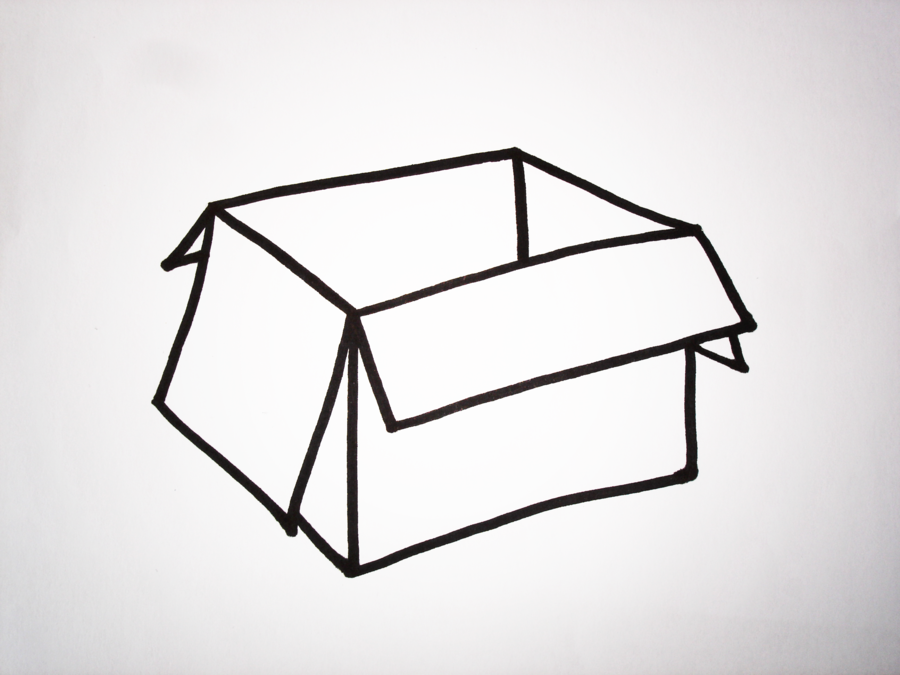
\includegraphics[width=\textwidth]{fig/empty_box}
			\caption{Sous-figure 1}
	\end{subfigure}
	\begin{subfigure}[b]{0.45\textwidth}
		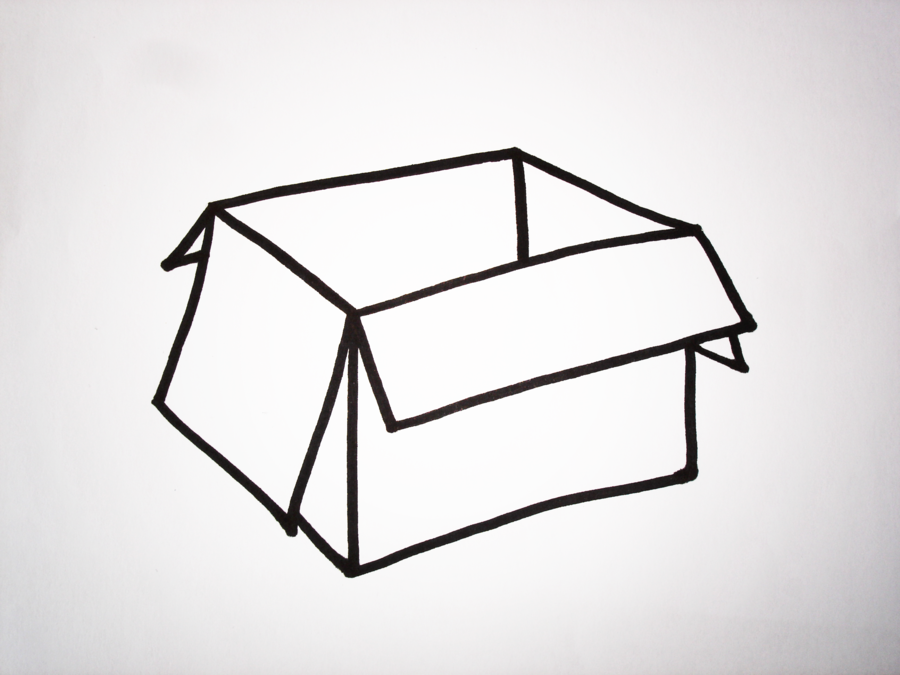
\includegraphics[width=\textwidth]{fig/empty_box}
			\caption{Sous-figure 2}
	\end{subfigure}
    \caption{Titre de la figure.}
	\legend{
		Lorem ipsum dolor sit amet, consectetur adipiscing elit. Sed tortor quam, facilisis in magna at, convallis fringilla risus. Curabitur; adipiscing: imperdiet ligula ut congue.
	}
    \label{fig:x}
\end{figure}

Phasellus vitae orci ac tellus accumsan rutrum et rutrum elit. Phasellus accumsan nunc quam, a bibendum felis posuere quis. Ut dui turpis, consequat sit amet felis in, imperdiet aliquam elit. Aliquam eget iaculis nisl, eu lobortis eros. Nunc euismod eros eu felis tristique congue. Morbi aliquam sapien lacus, non viverra eros venenatis sit amet. Aliquam erat volutpat. Vestibulum arcu elit, fringilla in ornare in, mattis sed nisl. Nunc cursus sem odio, at convallis nulla egestas vitae. Sed euismod semper ante eget egestas. Nulla aliquam nisl eu dui lobortis, sed euismod sem tincidunt. Proin laoreet risus dolor, vel commodo turpis lobortis eu. Quisque luctus at arcu eget hendrerit. Sed dapibus risus condimentum mauris accumsan, a scelerisque lorem tristique. Duis at vulputate augue. Integer diam mauris, condimentum eu odio sed, pellentesque gravida odio.

Référence : \citep{test2014}

Donec vitae malesuada odio. Vestibulum ante ipsum primis in faucibus orci luctus et ultrices posuere cubilia Curae; Fusce est massa, aliquet ut cursus quis, porttitor at leo. Etiam consectetur nulla mi, et ultricies tortor elementum eget. Vestibulum in purus accumsan, ullamcorper libero in, rutrum risus. Quisque non pellentesque mi. In hac habitasse platea dictumst. Sed facilisis non dolor quis porta. Vivamus ornare eget sem nec sollicitudin. Ut a purus fringilla, fringilla elit et, varius lectus. Proin et mauris odio.

\begin{table}[htb]
\caption{Légende du tableau}
\label{tab:x}
\centering
  \newcolumntype{L}[1]{>{\raggedright\arraybackslash}X}
  \newcolumntype{C}[1]{>{\hsize=#1\centering\arraybackslash}X}
  \begin{tabularx}{8cm}{C{5cm} L{}}
    \hline
    Colonne 1 & Colonne 2\\
    \hline
    un & 1\\
    deux & 2\\
    trois & 3\\
    quatre & 4\\
    cinq & 5\\
  \end{tabularx}
\end{table}


Sed tincidunt semper pharetra. Sed sodales erat in tristique interdum. Interdum et malesuada fames ac ante ipsum primis in faucibus. Integer bibendum lorem ipsum, vel dapibus dolor semper convallis. Sed vitae orci vitae lacus elementum pellentesque. Pellentesque tincidunt odio et purus placerat, id vulputate nulla convallis. Fusce pellentesque egestas enim, vitae tempor nulla egestas eget. Donec pretium ipsum vitae egestas dapibus.

Integer non tincidunt risus, id placerat quam. Proin aliquet odio nec augue ornare, in varius lectus dictum. Donec tincidunt imperdiet nisl, eget sagittis tellus tempor dignissim. Morbi pharetra sagittis justo, eu pharetra justo adipiscing sed. Praesent viverra nunc dolor, at eleifend erat vehicula a. Nam suscipit est id dui consequat vehicula. Etiam cursus blandit turpis, a adipiscing dui. Morbi leo mauris, convallis vitae aliquam a, commodo quis ante. Donec et pulvinar nisi. Ut aliquet odio ligula, a fringilla nisi sagittis id. Curabitur vitae diam vitae quam rhoncus varius sit amet quis diam. Fusce eget arcu sed arcu sagittis mattis. Cras non vehicula enim, id lobortis augue.

\section{Revue de littérature}
Quisque eu orci ultrices eros scelerisque tincidunt quis in velit. Sed sed odio vel nulla accumsan pulvinar ac quis ante. Ut pharetra nisl feugiat, ultricies lectus sit amet, aliquam magna. In hac habitasse platea dictumst. Morbi suscipit sagittis finibus. In hac habitasse platea dictumst. Maecenas ut quam orci. Etiam finibus ante enim, quis gravida nunc gravida sit amet. Curabitur pharetra arcu vitae erat convallis blandit. Cras pharetra faucibus mi nec venenatis. Suspendisse eget mollis odio, vel ornare augue. Suspendisse consequat fringilla diam, eget interdum quam placerat nec. Duis eleifend venenatis libero, at hendrerit enim sollicitudin a. Phasellus eu tortor eget tortor dictum aliquam. Nam a sem vel urna hendrerit ornare. In hac habitasse platea dictumst.

\subsection{Sous-section}
Sed pellentesque tempus pellentesque. Nulla efficitur laoreet dolor posuere ultricies. Donec viverra vehicula elit et euismod. Aliquam eu imperdiet augue, eu gravida eros. Nam in justo diam. Etiam in lorem congue, ullamcorper felis sit amet, tempor urna. Nulla ipsum nisl, commodo id aliquam sit amet, bibendum ut nisi. Donec diam massa, interdum pellentesque commodo at, euismod lacinia nisi. Vivamus sagittis sollicitudin sem ac tempor.

\paragraph{Sous-sous-section\\}
Nam vitae arcu sit amet tortor efficitur pretium ut eget sem. Vestibulum accumsan tortor in elit vehicula auctor. Maecenas et mauris egestas, efficitur massa fermentum, vestibulum arcu. Nulla id porttitor mauris. Phasellus non posuere risus. Donec sit amet urna urna. Cras finibus vitae justo eget lobortis.

\section{Structure de la thèse}
Donec rhoncus tempor mollis. Nulla tristique quam vel convallis rutrum. Sed egestas cursus mauris, ac rhoncus erat lobortis at. Mauris gravida lacinia ullamcorper. Etiam at sem leo. Proin pellentesque, orci ac finibus aliquet, erat mi vehicula libero, id cursus sem arcu eu quam. Integer dapibus ipsum et magna porta consectetur.

%!TEX root = ../main.tex
\chapter{Discussion}
Cette partie constituée d’un chapitre final contenant une discussion générale et une conclusion. La discussion générale sert d’abord à synthétiser les éléments principaux présentés dans les articles et à les mettre en relation. Cette discussion permet aussi de faire ressortir les éléments originaux et novateurs de la recherche, d’identifier les éventuelles limites des travaux, et de présenter des perspectives pour des travaux futurs. Ce chapitre final devrait typiquement comporter une vingtaine de pages.

\section{Section}
Lorem ipsum dolor sit amet, consectetur adipiscing elit. Sed tortor quam, facilisis in magna at, convallis fringilla risus. Curabitur adipiscing imperdiet ligula ut congue. Nunc non urna sed velit aliquet tempor. Fusce tempus vestibulum pharetra. Sed laoreet erat sed odio cursus, et egestas lacus fringilla. Nullam sollicitudin condimentum scelerisque. Morbi fermentum blandit purus, eget feugiat quam egestas at. Nam at velit ac velit feugiat lacinia. Mauris quis tortor dignissim, feugiat justo eget, interdum tortor. Proin vel lacus non eros eleifend aliquet nec at elit. Integer rhoncus laoreet ligula.

\section{Conclusion}

Morbi auctor lobortis lectus vel hendrerit. Nunc faucibus lacinia est ac semper. Quisque sodales nulla vitae urna tristique, sed vestibulum orci viverra. Ut consectetur dui lectus, vel porttitor ante dictum eget. Sed accumsan nec risus vitae aliquet. Vivamus scelerisque, sapien quis porta ultrices, urna lorem suscipit risus, id blandit diam mi et magna. Quisque leo nunc, lobortis sit amet imperdiet ac, vestibulum sed dolor. Aenean non sollicitudin nunc. Sed tempor libero vitae erat venenatis, sit amet semper diam interdum. Morbi eu aliquam lectus. Suspendisse potenti. Curabitur non iaculis augue. Curabitur felis est, dapibus id mauris eget, pharetra viverra libero. Donec vel nisi vitae turpis vehicula euismod eget in lectus. Praesent ut varius mauris.

\chapter{Lorem ipsum}

Lorem ipsum dolor sit amet, consectetur adipiscing elit. Sed tortor quam, facilisis in magna at, convallis fringilla risus. Curabitur adipiscing imperdiet ligula ut congue. Nunc non urna sed velit aliquet tempor. Fusce tempus vestibulum pharetra. Sed laoreet erat sed odio cursus, et egestas lacus fringilla. Nullam sollicitudin condimentum scelerisque. Morbi fermentum blandit purus, eget feugiat quam egestas at. Nam at velit ac velit feugiat lacinia. Mauris quis tortor dignissim, feugiat justo eget, interdum tortor. Proin vel lacus non eros eleifend aliquet nec at elit. Integer rhoncus laoreet ligula.

% Omettre si thèse/mémoire traditionnel
\part{Articles}
\renewcommand{\chaptername}{Article} % Afficher "Article" plutôt que "Chapitre".
\setcounter{chapter}{0} % Recommencer la numérotation des chapitres.
\chapter{Lorem ipsum}
\chaptermark{Lorem} % Titre court apparaissant dans l'entête des pages

{\setlength{\parindent}{0cm}
\textbf{Titre traduit}
\\ Lorem ipsum

\textbf{Auteurs}
\\Prénom Nom$^1$, Prénom Nom$^2$
\\$^1$ Affiliation
\\$^2$ Affiliation

\textbf{Contribution}
\\Lorem ipsum dolor sit amet, consectetur adipiscing elit. Sed tortor quam, facilisis in magna at, convallis fringilla risus. Curabitur adipiscing imperdiet ligula ut congue. Nunc non urna sed velit aliquet tempor. Fusce tempus vestibulum pharetra. Sed laoreet erat sed odio cursus, et egestas lacus fringilla. Nullam sollicitudin condimentum scelerisque. Morbi fermentum blandit purus, eget feugiat quam egestas at. Nam at velit ac velit feugiat lacinia. Mauris quis tortor dignissim, feugiat justo eget, interdum tortor. Proin vel lacus non eros eleifend aliquet nec at elit. Integer rhoncus laoreet ligula.

\textbf{Publication ciblée}
\\Journal
\\Date de soumission

\textbf{Résumé traduit}
\\Lorem ipsum dolor sit amet, consectetur adipiscing elit. Sed tortor quam, facilisis in magna at, convallis fringilla risus. Curabitur adipiscing imperdiet ligula ut congue. Nunc non urna sed velit aliquet tempor. Fusce tempus vestibulum pharetra. Sed laoreet erat sed odio cursus, et egestas lacus fringilla. Nullam sollicitudin condimentum scelerisque. Morbi fermentum blandit purus, eget feugiat quam egestas at. Nam at velit ac velit feugiat lacinia. Mauris quis tortor dignissim, feugiat justo eget, interdum tortor. Proin vel lacus non eros eleifend aliquet nec at elit. Integer rhoncus laoreet ligula.
}

\section{Lorem ipsum}
Lorem ipsum dolor sit amet, consectetur adipiscing elit. Sed tortor quam, facilisis in magna at, convallis fringilla risus. Curabitur adipiscing imperdiet ligula ut congue. Nunc non urna sed velit aliquet tempor. Fusce tempus vestibulum pharetra. Sed laoreet erat sed odio cursus, et egestas lacus fringilla. Nullam sollicitudin condimentum scelerisque. Morbi fermentum blandit purus, eget feugiat quam egestas at. Nam at velit ac velit feugiat lacinia. Mauris quis tortor dignissim, feugiat justo eget, interdum tortor. Proin vel lacus non eros eleifend aliquet nec at elit. Integer rhoncus laoreet ligula.

\section{Lorem ipsum}
Donec vitae malesuada odio. Vestibulum ante ipsum primis in faucibus orci luctus et ultrices posuere cubilia Curae; Fusce est massa, aliquet ut cursus quis, porttitor at leo. Etiam consectetur nulla mi, et ultricies tortor elementum eget. Vestibulum in purus accumsan, ullamcorper libero in, rutrum risus. Quisque non pellentesque mi. In hac habitasse platea dictumst. Sed facilisis non dolor quis porta. Vivamus ornare eget sem nec sollicitudin. Ut a purus fringilla, fringilla elit et, varius lectus. Proin et mauris odio.

\section{Lorem ipsum}
Integer non tincidunt risus, id placerat quam. Proin aliquet odio nec augue ornare, in varius lectus dictum. Donec tincidunt imperdiet nisl, eget sagittis tellus tempor dignissim. Morbi pharetra sagittis justo, eu pharetra justo adipiscing sed. Praesent viverra nunc dolor, at eleifend erat vehicula a. Nam suscipit est id dui consequat vehicula. Etiam cursus blandit turpis, a adipiscing dui. Morbi leo mauris, convallis vitae aliquam a, commodo quis ante. Donec et pulvinar nisi. Ut aliquet odio ligula, a fringilla nisi sagittis id. Curabitur vitae diam vitae quam rhoncus varius sit amet quis diam. Fusce eget arcu sed arcu sagittis mattis. Cras non vehicula enim, id lobortis augue.

\singlespacing
\cleardoublepage
\phantomsection
\renewcommand{\bibname}{Références} % Afficher "Références" plutôt que "Bibliographie".
\addcontentsline{toc}{chapter}{\bibname} % Ajouter une ligne pour la bibliographie dans la table des matières.
\bibliographystyle{bibliostyleINRS} % Utiliser le style bibliographique de l'INRS.
\bibliography{biblio/biblio} % Générer la bibliographie avec Bibtex (fichier biblio.bib).
%\include{biblio/biblio} % Inclure une bibliographie écrite manuellement.

% Si désiré, ajouter des annexes.
\appendix
%!TEX root = ../main.tex
\chapter{Annexe I: Les pages annexes}
Les pages annexes apportent un complément d’information au corps du travail et ne doivent contenir que ce qui est important pour la compréhension de la thèse ou ce qui en supporte l’argumentation. Il est important de ne pas inclure n’importe quoi dans les annexes simplement pour sauver du temps, en se rappelant qu’elles seront publiées sur internet.

Les annexes sont placées après la bibliographie. S’il y en a plusieurs, elles sont présentées selon l’ordre de mention dans le texte avec la numérotation Annexe I, Annexe II, Annexe III, etc. Numérotation en chiffres romains majuscules suivie de leur propre titre.

D’autres listes peuvent être ajoutées au besoin. Par exemple, liste des publications ou documents inclus dans le texte ou hors texte, d’abréviations, sigles ou symboles, d’annexes, etc.

\section{Lorem ipsum}
Lorem ipsum dolor sit amet, consectetur adipiscing elit. Sed tortor quam, facilisis in magna at, convallis fringilla risus. Curabitur adipiscing imperdiet ligula ut congue. Nunc non urna sed velit aliquet tempor. Fusce tempus vestibulum pharetra. Sed laoreet erat sed odio cursus, et egestas lacus fringilla. Nullam sollicitudin condimentum scelerisque. Morbi fermentum blandit purus, eget feugiat quam egestas at. Nam at velit ac velit feugiat lacinia. Mauris quis tortor dignissim, feugiat justo eget, interdum tortor. Proin vel lacus non eros eleifend aliquet nec at elit. Integer rhoncus laoreet ligula.


\end{document}
